% Slide 6: KNN Regression Problem
\begin{frame}{بیان مسئله در رگرسیون $k$ نزدیک‌ترین همسایه}{\lr{K-Nearest-Neighbors Regression}}
  \begin{columns}[T]
    \begin{column}{0.54\textwidth}
      \begin{itemize}
        \setlength{\itemsep}{8pt}
        \item \textbf{بیان مسئله:} (\lr{Problem})
        \begin{itemize}
          \setlength{\itemsep}{5pt}
          \item پیش‌بینی دمای هوا در یک موقعیت جغرافیایی خاص ($x$).
          \item در نقطه‌ای که هیچ ایستگاه هواشناسی در آنجا مستقر نیست!
          \item چگونه می‌توان چنین پیش‌بینی پیوسته‌ای را انجام داد؟
        \end{itemize}
        \item ایده طبیعی: استفاده از اطلاعات نزدیک‌ترین ایستگاه‌های هواشناسی مجاور.
      \end{itemize}
    \end{column}
    \begin{column}{0.44\textwidth}
      \begin{center}
        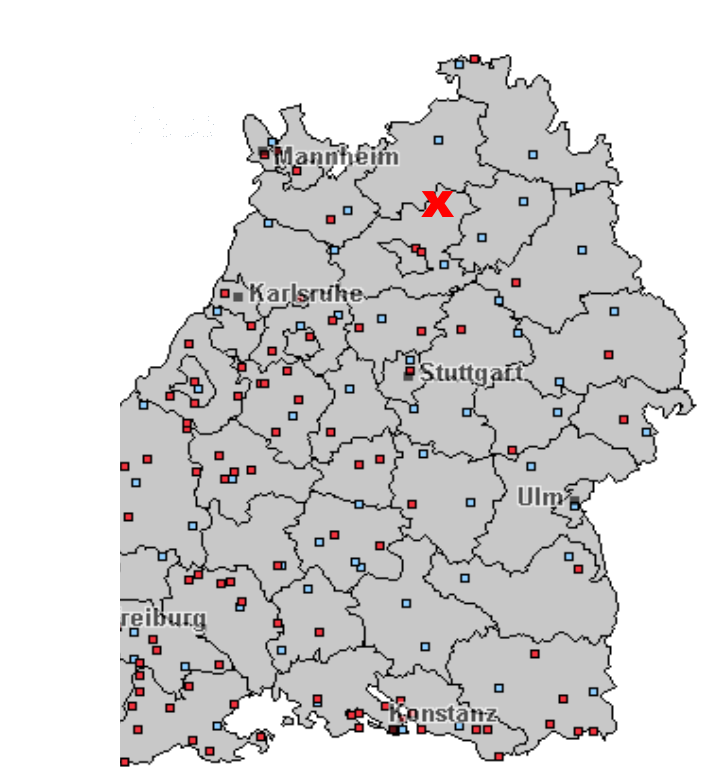
\includegraphics[width=\textwidth,height=4.6cm,keepaspectratio]{images/slide06_knn_regression.png}
      \end{center}
    \end{column}
  \end{columns}
\end{frame}

% Slide 7: Recap KNN Classification
\begin{frame}{یادآوری: طبقه‌بندی $k$ نزدیک‌ترین همسایه}{\lr{Recap: K-Nearest-Neighbors Classification}}
  \begin{columns}[T]
    \begin{column}{0.54\textwidth}
      \begin{itemize}
        \setlength{\itemsep}{5pt}
        \item \textbf{ایده در طبقه‌بندی:} رأی‌گیری اکثریت (\lr{Majority Vote}) میان نزدیک‌ترین ایستگاه‌ها.
        \item \textbf{مثال طبقه‌بندی:}
        \begin{itemize}
          \item ۳ ایستگاه: ابری (\lr{Cloudy})
          \item ۲ ایستگاه: آفتابی (\lr{Sunny})
          \item \textbf{نتیجه رأی‌گیری:} ابری (\lr{Cloudy})
        \end{itemize}
        \item پارامتر $k$ تعداد همسایگان مدنظر را تعیین می‌کند ($k=5$).
        \item «نزدیکی» بر مبنای مجاورت جغرافیایی یا فاصله اقلیدسی تعریف می‌شود.
      \end{itemize}
    \end{column}
    \begin{column}{0.44\textwidth}
      \begin{center}
        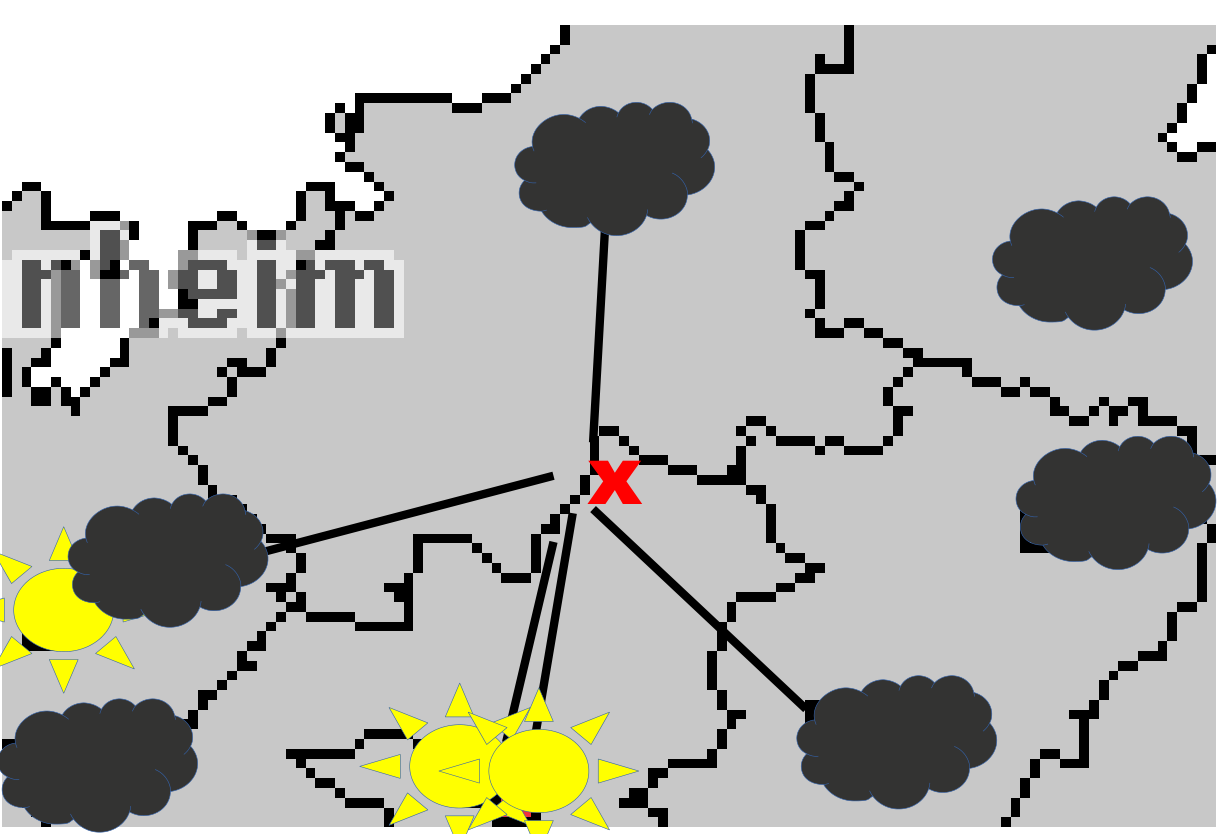
\includegraphics[width=\textwidth,height=3.8cm,keepaspectratio]{images/slide07_recap_knn.png}
      \end{center}
    \end{column}
  \end{columns}
\end{frame}

% Slide 8: KNN Regression Concept
\begin{frame}{برآورد عددی در رگرسیون $k$ نزدیک‌ترین همسایه}{\lr{K-Nearest-Neighbors Regression}}
  \begin{columns}[T]
    \begin{column}{0.53\textwidth}
      \begin{itemize}
        \setlength{\itemsep}{5pt}
        \item \textbf{ایده در رگرسیون:} استفاده از \textbf{میانگین عددی} مقادیر ایستگاه‌های مجاور.
        \item \textbf{مثال محاسباتی} ($k=5$):
        \begin{itemize}
          \item دماهای ثبت‌شده: $18^\circ\mathrm{C}, 20^\circ\mathrm{C}, 21^\circ\mathrm{C}, 22^\circ\mathrm{C}, 21^\circ\mathrm{C}$
        \end{itemize}
      \end{itemize}
      \vspace{-0.1cm}
      \begin{center}
        $\displaystyle \hat{y} = \frac{18 + 20 + 21 + 22 + 21}{5} = \mathbf{20.4^\circ\mathrm{C}}$
      \end{center}
      \vspace{-0.1cm}
      \begin{itemize}
        \item \textbf{میانگین‌گیری وزنی بر اساس فاصله:}
        ایستگاه‌های نزدیک‌تر وزن بیشتری در تعیین مقدار خروجی دارند.
      \end{itemize}
    \end{column}
    \begin{column}{0.45\textwidth}
      \begin{center}
        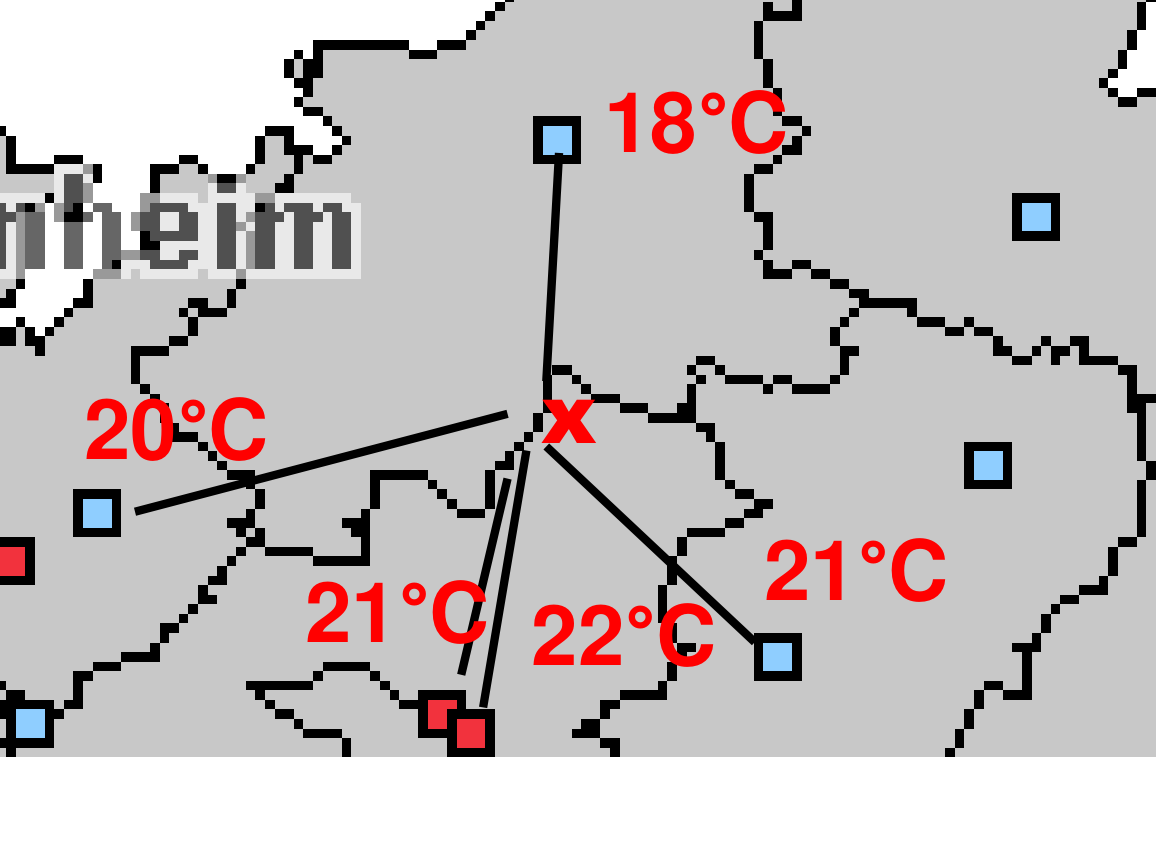
\includegraphics[width=\textwidth,height=4.0cm,keepaspectratio]{images/slide08_weather_stations.png}
      \end{center}
    \end{column}
  \end{columns}
\end{frame}

% Slide 9: Python Implementation
\begin{frame}{پیاده‌سازی رگرسیون $k$ نزدیک‌ترین همسایه در پایتون}{\lr{K-NN Regression in Scikit-Learn}}
  \begin{columns}[T]
    \begin{column}{0.58\textwidth}
      \begin{latin}
        \begin{minipage}{\textwidth}
          \fcolorbox{codeborder}{codebg}{%
            \begin{minipage}{0.96\textwidth}
              {\fontsize{6.8}{9.0}\selectfont\ttfamily
              \textcolor{blue}{\textbf{from}} sklearn.neighbors \textcolor{blue}{\textbf{import}} KNeighborsRegressor\\[0.15cm]
              \textcolor{mannheimteal}{\# 1. Create and fit KNN regressor}\\
              estimator = KNeighborsRegressor(n\_neighbors=15)\\[0.05cm]
              estimator.fit(training\_set\_X, training\_dependent\_y)\\[0.15cm]
              \textcolor{mannheimteal}{\# 2. Predict for unseen examples}\\
              y\_hat = estimator.predict(test\_set\_X)
              }
            \end{minipage}%
          }
        \end{minipage}
      \end{latin}
      \vspace{0.25cm}
      {\fontsize{8.5}{11}\selectfont
      \begin{itemize}
        \setlength{\itemsep}{4pt}
        \item \textbf{وزن‌دهی یکنواخت} (\lr{uniform})؛ میانگین ساده حسابی مقادیر همسایگان.
        \item \textbf{وزن‌دهی بر مبنای فاصله} (\lr{distance})؛ اختصاص وزن بیشتر بر مبنای معکوس فاصله نمونه‌ها.
      \end{itemize}
      }
    \end{column}
    \begin{column}{0.40\textwidth}
      \begin{center}
        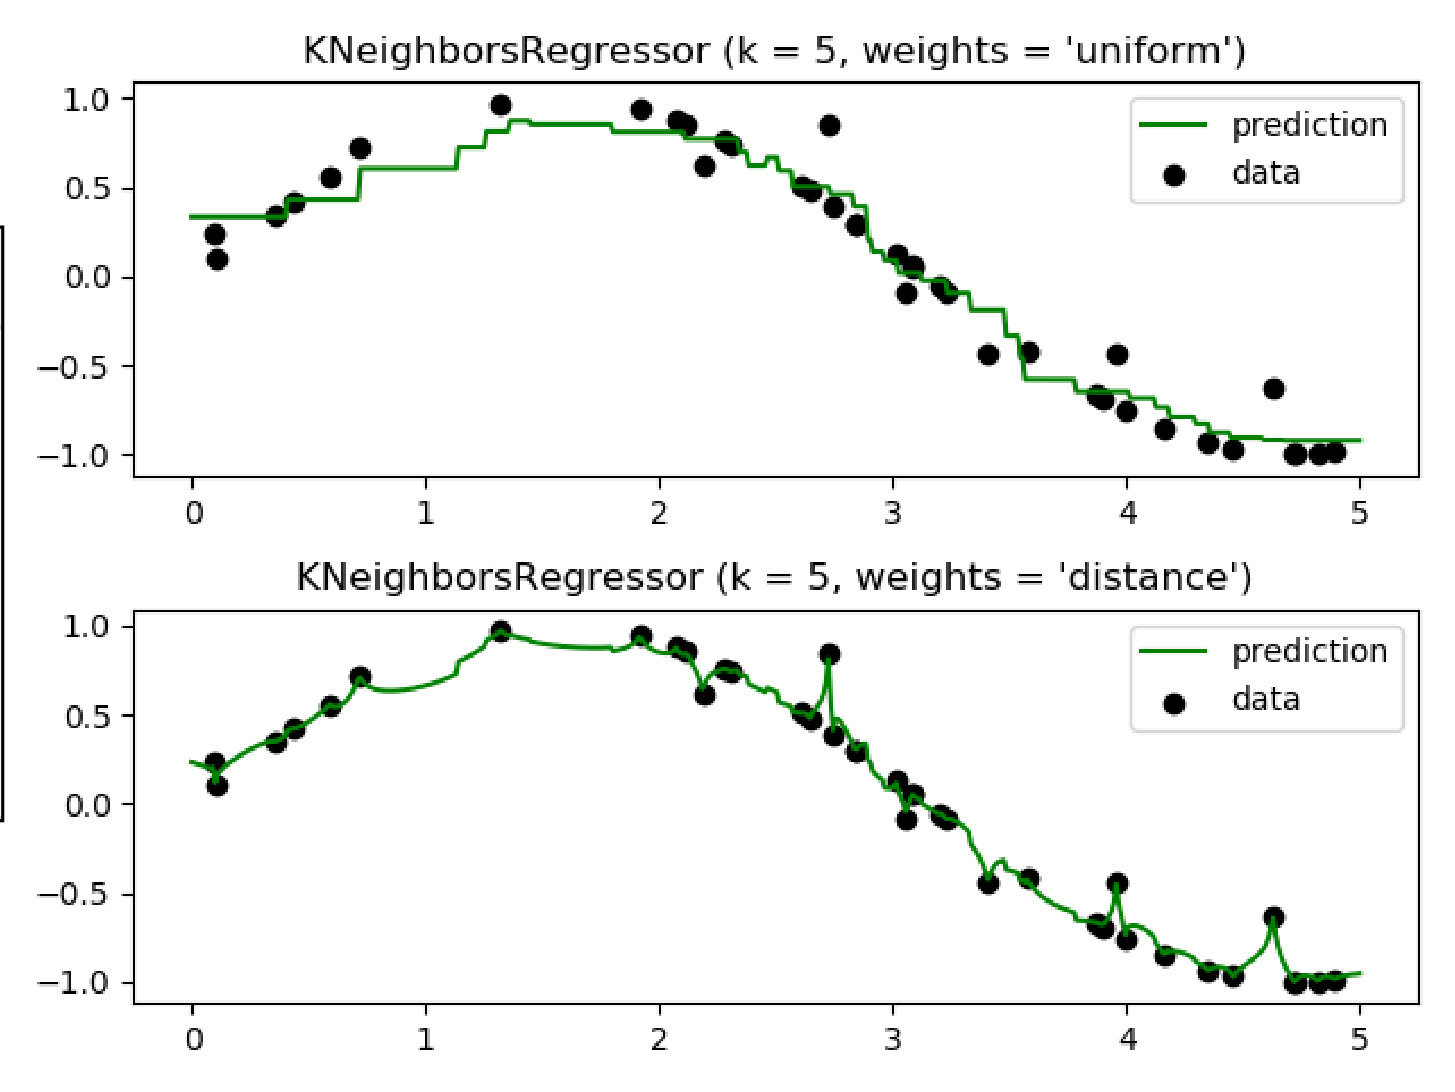
\includegraphics[width=\textwidth,height=4.5cm,keepaspectratio]{images/slide09_knn_prediction_curves.png}
      \end{center}
    \end{column}
  \end{columns}
\end{frame}

% Slide 10: Evaluation Metrics - MAE, MSE, RMSE
\begin{frame}{معیارهای ارزیابی خطا (\lr{MAE, MSE, RMSE})}{\lr{Evaluation Metrics: Error Measures}}
  \begin{itemize}
    \setlength{\itemsep}{2pt}
    \item \textbf{میانگین قدرمطلق خطا:} (\lr{MAE}) میانگین اختلاف بین مقدار پیش‌بینی ($p_i$) و مقدار واقعی ($a_i$) است.
    \vspace{-0.15cm}
    \[
      \text{MAE} = \frac{1}{n} \sum_{i=1}^n |p_i - a_i| \qquad \text{\small(هم‌مقیاس با دامنه مسئله، مانند دما)}
    \]
    \vspace{-0.15cm}
    \item \textbf{میانگین مربعات خطا:} (\lr{MSE}) خطاهای بزرگ‌تر را با شدت بیشتری جریمه می‌کند.
    \vspace{-0.15cm}
    \[
      \text{MSE} = \frac{1}{n} \sum_{i=1}^n (p_i - a_i)^2
    \]
    \vspace{-0.15cm}
    \item \textbf{جذر میانگین مربعات خطا:} (\lr{RMSE}) دارای مقیاس یکسان با متغیر هدف و تأکید بیشتر بر خطاهای بزرگ.
    \vspace{-0.15cm}
    \[
      \text{RMSE} = \sqrt{\text{MSE}} = \sqrt{\frac{1}{n} \sum_{i=1}^n (p_i - a_i)^2} \qquad \text{\small(هم‌مقیاس با دامنه مسئله)}
    \]
  \end{itemize}
  \vspace{-0.25cm}
  \begin{center}
    {\fontsize{7.5}{9.5}\selectfont\color{subgray}\textbf{مقدار پیش‌بینی‌شده:} $p_i$ \lr{(Predicted)} \quad | \quad \textbf{مقدار واقعی:} $a_i$ \lr{(Actual)}}
  \end{center}
\end{frame}

% Slide 11: Pearson Correlation
\begin{frame}{معیارهای ارزیابی: ضریب همبستگی پیرسون}{\lr{Pearson's Correlation Coefficient (PCC)}}
  \begin{columns}[c]
    \begin{column}{0.73\textwidth}
      \begin{itemize}
        \setlength{\itemsep}{2pt}
        {\fontsize{8.5}{11}\selectfont
        \item مقدار نرمال‌شده در بازه \lr{$[-1, 1]$}
        \item امتیاز بالا زمانی حاصل می‌شود که:
        \begin{itemize}
          \item مقادیر واقعی بزرگ، پیش‌بینی‌های بزرگ دریافت کنند.
          \item مقادیر واقعی کوچک، پیش‌بینی‌های کوچک دریافت کنند.
        \end{itemize}
        \item \textbf{هشدار مهم:} ضریب پیرسون نسبت به مقیاس \textbf{ناوردا} (\lr{Scale-Invariant}) است!
        \begin{itemize}
          \item درآمد واقعی برابر \lr{\$1, \$2, \$3}
          \item درآمد پیش‌بینی‌شده برابر \lr{\$1,000, \$2,000, \$3,000}
          \item نتیجه به دست آمده: \lr{$\text{PCC} = 1$} (علیرغم اختلاف فاحش در مقادیر مطلق!)
        \end{itemize}
        }
      \end{itemize}
    \end{column}
    \begin{column}{0.25\textwidth}
      \begin{center}
        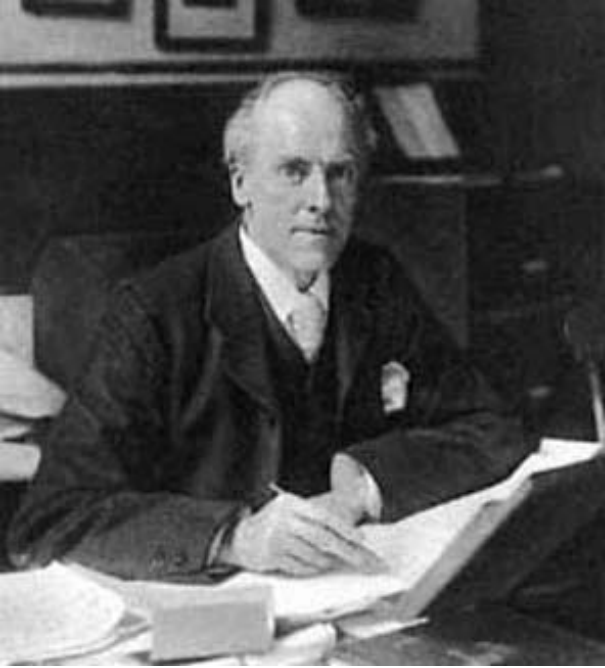
\includegraphics[width=\textwidth,height=2.3cm,keepaspectratio]{images/slide11_pearson_formula_diagram.png}\\[2pt]
        {\fontsize{6.5}{8}\selectfont\color{subgray}\lr{Karl Pearson (1857--1936)}}
      \end{center}
    \end{column}
  \end{columns}

  \vspace{0.1cm}
  \begin{columns}[c]
    \begin{column}{0.54\textwidth}
      \begin{center}
        {\fontsize{8.5}{11}\selectfont $\displaystyle \text{PCC} = \frac{\sum_{i=1}^n (p_i - \bar{p})(a_i - \bar{a})}{\sqrt{\sum_{i=1}^n (p_i - \bar{p})^2} \cdot \sqrt{\sum_{i=1}^n (a_i - \bar{a})^2}}$}
      \end{center}
    \end{column}
    \begin{column}{0.44\textwidth}
      \begin{center}
        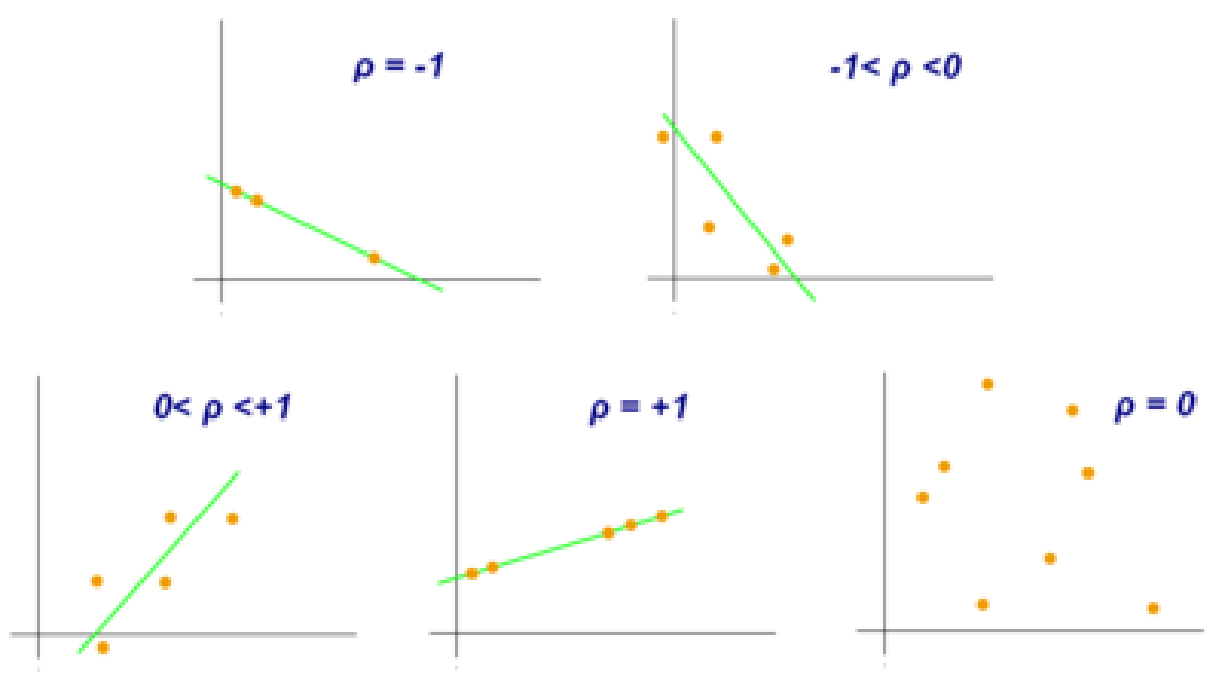
\includegraphics[width=\textwidth,height=2.0cm,keepaspectratio]{images/slide11_pearson_scatter_grid.png}
      \end{center}
    \end{column}
  \end{columns}
\end{frame}

% Slide 12: R-Squared
\begin{frame}{معیارهای ارزیابی: ضریب تعیین}{\lr{Coefficient of Determination ($R^2$)}}
  \begin{columns}[T]
    \begin{column}{0.56\textwidth}
      \begin{itemize}
        \setlength{\itemsep}{3pt}
        \item مقداری نرمال‌شده در بازه \lr{$[0, 1]$} (برای مدل‌های معقول).
        \item بیانگر سهمی از کل تغییرات متغیر وابسته $y$ که توسط متغیرهای توصیفی $X$ تبیین‌پذیر است:
      \end{itemize}
      \vspace{-0.1cm}
      \begin{center}
        {\fontsize{8.5}{11}\selectfont $\displaystyle R^2 = \frac{\sum_{i=1}^n (p_i - \bar{a})^2}{\sum_{i=1}^n (a_i - \bar{a})^2} = \frac{\text{ESS}}{\text{TSS}}$}
      \end{center}
      \vspace{-0.1cm}
      \begin{itemize}
        \setlength{\itemsep}{2pt}
        \item \textbf{تفسیر مقادیر $R^2$}:
        \begin{itemize}
          \item به ازای $R^2 = 1$: مدل ایده‌آل؛ کل پراکندگی $y$ به طور کامل توسط $X$ توضیح داده شده است.
          \item به ازای $R^2 = 0$: مدل در حد خط پایه (میانگین $\bar{a}$) عمل می‌کند.
        \end{itemize}
      \end{itemize}
    \end{column}
    \begin{column}{0.42\textwidth}
      \begin{center}
        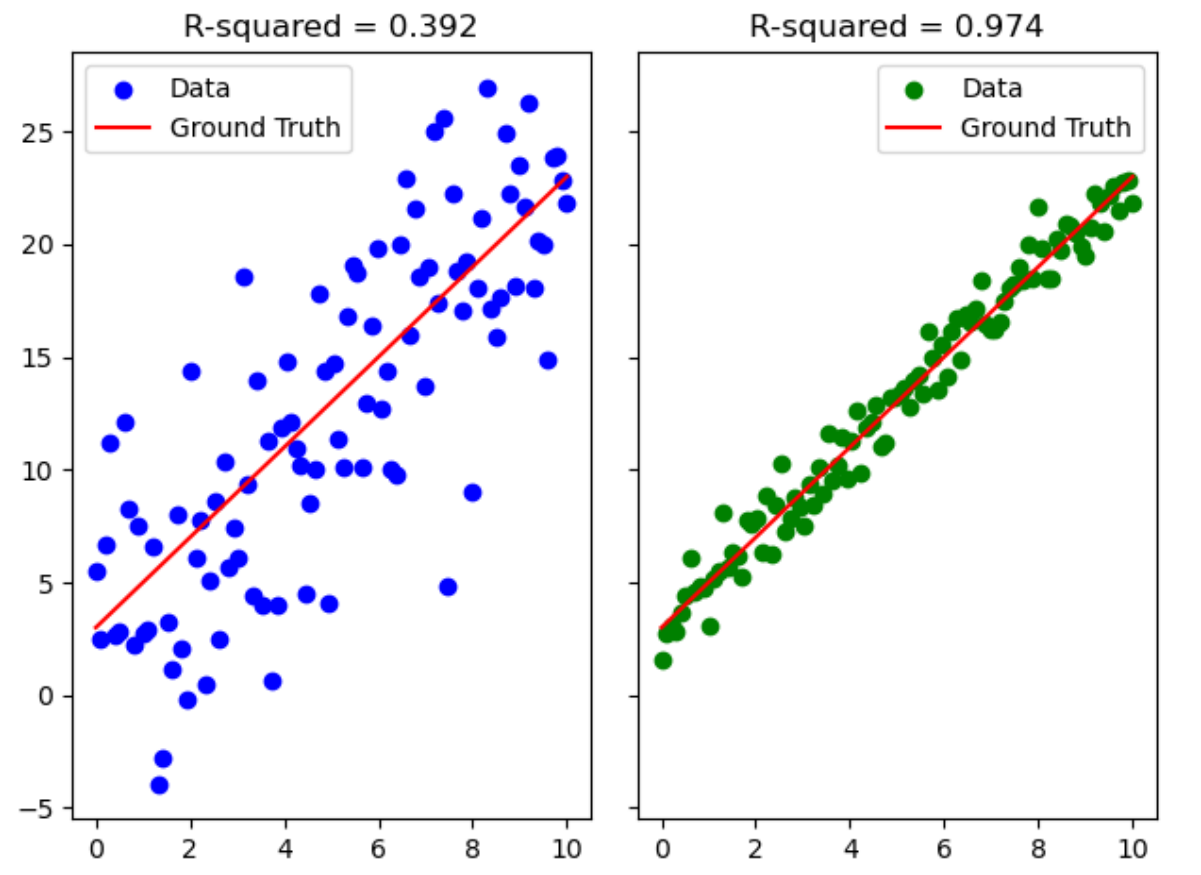
\includegraphics[width=\textwidth,height=4.0cm,keepaspectratio]{images/slide12_r2_tss_rss_diagram.png}
      \end{center}
    \end{column}
  \end{columns}
\end{frame}
